% Created 2011-08-12 Fri 19:27
% BEGIN My Article Defaults
    \documentclass[10pt,letterpaper]{article}
    
    \usepackage[letterpaper,includeheadfoot,top=0.5in,bottom=0.5in,left=0.75in,right=0.75in]{geometry}
    \usepackage[utf8]{inputenc}
    \usepackage[T1]{fontenc}
    \usepackage{hyperref}
    \usepackage{lastpage}
    \usepackage{fancyhdr}
    \usepackage[all]{xy}              %for doing graphics http://en.wikibooks.org/wiki/LaTeX/Creating_Graphics#Xy-pic
    \pagestyle{fancy}
    \renewcommand{\headrulewidth}{1pt}
    \renewcommand{\footrulewidth}{0.5pt}
    
    % For the engineering phasor symbol
    % http://newsgroups.derkeiler.com/Archive/Comp/comp.text.tex/2006-02/msg00895.html
    \makeatletter
    \def\phase#1{{\vbox{\ialign{$\m@th\scriptstyle##$\crcr
    \not\mathrel{\mkern10mu\smash{#1}}\crcr
    \noalign{\nointerlineskip}
    \mkern2.5mu\leaders\hrule height.34pt\hfill\mkern2.5mu\crcr}}}}
    \makeatother
    
    % Default footer
    \fancyfoot[L]{\small \jobname \\ \today}
    \fancyfoot[C]{\small Page \thepage\ of \pageref{LastPage}}
    \fancyfoot[R]{\small \copyright \the\year\  Chris Beard}
    % END My Article Defaults
    
    
\usepackage[utf8]{inputenc}
\usepackage[T1]{fontenc}
\usepackage{fixltx2e}
\usepackage{graphicx}
\usepackage{longtable}
\usepackage{float}
\usepackage{wrapfig}
\usepackage{soul}
\usepackage{textcomp}
\usepackage{marvosym}
\usepackage[integrals]{wasysym}
\usepackage{latexsym}
\usepackage{amssymb}
\usepackage{hyperref}
\tolerance=1000
\usepackage{amsmath}
\providecommand{\alert}[1]{\textbf{#1}}
\begin{document}



\title{Linear Algebra Notes}
\author{Chris Beard}
\date{12 August 2011}
\maketitle

\setcounter{tocdepth}{3}
\tableofcontents
\vspace*{1cm}


\section{Linear Algebra Notes}
\label{sec-1}
\subsection{Basic Linear Algebra concepts}
\label{sec-1_1}

\begin{enumerate}
\setcounter{enumi}{12}
\item  Singular matrix, no inverse for matrix $M$; $|M|=0 \Leftrightarrow M ^{-1}$ undefined 13
\item Line: $L=\{\vec{x}+t \vec{v} | t \in \mathbb{R} \}$
\setcounter{enumi}{17}
\item  Set of $n$ linear independent vectors $\mathcal{V}=\{\vec{v}_1,\vec{v}_2,...,\vec{v}_n\}$:

\begin{itemize}
\item $c_1 \vec{v}_1 + c_2 \vec{v}_2 + ... + c_n \vec{v}_n=0 \Rightarrow c_1=c_2=...=c_n=0$
\item otherwise, $\mathcal{V}$ is linearly dependent
\end{itemize}

\item Subspace: vector space

\begin{itemize}
\item Span of $n$ vectors is valid subspace of $\mathbb{R}^n$
\item Subspace must be closed under addition
\item and scalar multiplication

\begin{itemize}
\item must include $\{\vec{0}\}$
\end{itemize}

\end{itemize}

\item Basis: minimum set of linearly independent vectors that spans a subspace
\item Dot product: $\vec{a} \cdot \vec{v}=a_1 v_1 + a_2 v_2 + ... + a_n v_n$

\begin{itemize}
\item commutative
\item distributive
\item associative
\end{itemize}

\setcounter{enumi}{22}
\item  Cauchy-Schwartz inequality

\begin{itemize}
\item $| \vec{x} \cdot \vec{y}| \le \| \vec{x} \| \| \vec{y} \|$
\item special case: $\vec{x}=c \vec{y} \Leftrightarrow | \vec{x} \cdot \vec{y}| = \| \vec{x} \| \| \vec{y} \|$
\end{itemize}

\item Vector triangle inequality

\begin{itemize}
\item $| \vec{x} + \vec{y}| \le \| \vec{x} \| + \| \vec{y} \|$
\item special case:  $| \vec{x} + \vec{y}| = \| \vec{x} \| + \| \vec{y} \| \Leftrightarrow \vec{x} = c \vec{y}$
\item simple, but helpful for scaling to general coordinates
\end{itemize}

\end{enumerate}
\subsection{Geometry}
\label{sec-1_2}


\begin{enumerate}
\item Angle $\theta$ between vectors

\begin{itemize}
\item $\vec{a} \cdot \vec{b} = \| \vec{a} \| \| \vec{b} \| \cos \theta$
\item $\vec{a} \perp \vec{b} \Rightarrow \vec{a} \cdot \vec{b} =0$
\end{itemize}

\item Find a plane

\begin{itemize}
\item $\vec{x}_0$ is a point on the plane, $\vec{n}$ is a vector normal to the plane, $\vec{x}$ is a vector that ends on the plane
\item get plane in traditional form: $Ax + By + Cz =D$

\begin{itemize}
\item via: $n_1(x-x_0) + n_2(y-y_0) + n_3(z-z_0)=0$
\end{itemize}

\end{itemize}

\setcounter{enumi}{28}
\item  Area of a parallelogram formed by vectors $\vec{a}, \vec{b}$

\begin{itemize}
\item $A = \| \vec{a} \times \vec{b} \|$
\end{itemize}

\end{enumerate}
\subsection{Nullspace $\mathcal{N}$}
\label{sec-1_3}

\begin{enumerate}
\setcounter{enumi}{33}
\item  Subspace: Nullspace $N = \{ \vec{x} \in \mathbb{R}^n | A \vec{x} = \vec{0} \}$

\begin{itemize}
\item $N(A)=N(rref(A))$
\item $N(A)=0 \Leftrightarrow$ column vectors are linearly independent
\end{itemize}

\setcounter{enumi}{35}
\item  $\mathcal{N}(A)=\{0\} \Leftrightarrow$ column vectors are linearly independent
\setcounter{enumi}{39}
\item  Any basis of a given span will have the same number of elements
\setcounter{enumi}{41}
\item  ${\bf dim} (C(A))= {\bf rank} (A)$ (for column space of $A,C(A)$)
\end{enumerate}
\subsection{Transformations}
\label{sec-1_4}

\begin{enumerate}
\setcounter{enumi}{46}
\item  Linear transformations of $x$ can be represented as $Ax$ for some matrix $A$

\begin{itemize}
\item linearity:

\begin{itemize}
\item $A(x+y)=Ax + Ay$
\item $A(\alpha x) = \alpha Ax$
\end{itemize}

\end{itemize}

\item Matrix product with any vector is a linear transformation

\begin{itemize}
\item any linear transformation can be represented as a matrix vector product
\end{itemize}

\setcounter{enumi}{50}
\item  $\mathcal{V}$ a subspace in $\mathbb{R}^{n}$

\begin{itemize}
\item $T: \mathbb{R}^{n} \rightarrow \mathbb{R}^{m}$

\begin{itemize}
\item $T(\mathcal{V})$ is image of $\mathcal{V}$ under $T$
\item $T(\mathbb{R}^{n})$ is image of actual `T'
\end{itemize}

\end{itemize}

\item $T:X\rightarrow Y$, $S$ is a subset of domain $Y$

\begin{itemize}
\item everything in $x \subseteq X$ maps to some place in $Y$
\item everything in $S \subseteq Y$ gets mapped to
\item $T^{-1}(S)$ is pre-image of $S$ under $T$
\item $T^{-1}(S)= \{ \vec{x} \in \mathbb{R}^{n} | T( \vec{x}) \in S\}$
\item ${\bf kernel} (T)= \{ \vec{x} \in \mathbb{R}^{n} | T( \vec{x}) = \{0\}\}$
\end{itemize}

\end{enumerate}

57,58. Rotation transformation
\begin{itemize}
\item rotation is a linear $\Leftrightarrow$ representable as matrix product.
\item Basic method for $\mathbb{R}^{3}$: represent rotation around $x$ axis with matrix $A$, then about $y$ axis with a matrix $B$, then about $z$ axis with matrix $C$. (do this on unit vectors to find $A, B, C$). The resulting transform on a vector $\vec{x}$ will be $C(B(A \vec{x} ))$
\item In $\mathbb{R}^{2}$:
\end{itemize}
\[
A=
\begin{bmatrix}
  \cos(\theta) & -\sin(\theta) \\
  \sin(\theta) & \cos(\theta)  \\
\end{bmatrix}
\]
\begin{itemize}
\item In $\mathbb{R}^{3}$, around $x$-axis:
\end{itemize}
\[
A=
\begin{bmatrix}
  1 & 0            & 0             \\
  0 & \cos(\theta) & -\sin(\theta) \\
  0 & \sin(\theta) & \cos(\theta)  \\
\end{bmatrix}
\]
\begin{enumerate}
\setcounter{enumi}{59}
\item  Projections of $\vec{x}$ onto space $L=\{c \vec{v} | c \in \mathbb{R} \}$

\begin{itemize}
\item $\displaystyle {\bf Proj}_L (\vec{x}) = \left(\frac{\vec{x} \cdot \vec{v} } {\vec{v} \cdot \vec{v}}\right) \vec{v} = \frac{\vec{x} \cdot \vec{v} } {\|\vec{v}\| ^2} \vec{v}$
\item easier with unit vector
\end{itemize}

\item Projections are easier if you have a normalized vector $\vec{u}= \frac{\vec{v}}{\| \vec{v}\|}$:

\begin{itemize}
\item \fbox{$\displaystyle {\bf Proj}_L (\vec{x}) = \left( \vec{x} \cdot \vec{u} \right) \vec{u}$} $=A \vec{x}$ , where $\vec{u}$ is a unit vector on $L$
\item if $\hat{u}=\begin{bmatrix} u_1 \\ u_2 \end{bmatrix}$, get $A_{n\times n}$ by applying the transformation ${\bf Proj}_L (\vec x)$ to each column in $I_n$
\end{itemize}

\setcounter{enumi}{62}
\item  Given $T( \vec{x} )= B_{l \times m} \vec{x}, S(\vec{x})= A_{m\times n} \vec{x}$

\begin{itemize}
\item Then $T$ composed with $S$ is given as $T \circ S (\vec{x}) = T(S( \vec{x})) = B(A \vec{x})$
\item Remember interpretation of matrix vector products:
      $$ A \vec{x} = \begin{bmatrix} \vec{a}_1 & \vec{a}_2 & \cdots & \vec{a}_n \end{bmatrix} \begin{bmatrix} x_1 \\ x_2 \\  \vdots \\ x_n \end{bmatrix} = x_1 \vec{a}_1 + x_2 \vec{a}_2 + ... + x_n \vec{a}_n$$
\item In other words, the product of a matrix $A$ and a vector $\vec{x}$ is a \fbox{linear combination of the column matrices} of $A$, $\vec{a}_i$, scaled by the elements of $\vec{x}$, $x_i$
\end{itemize}

\end{enumerate}
\subsection{Invertibility}
\label{sec-1_5}

\begin{enumerate}
\setcounter{enumi}{66}
\item  Function $f$ is invertible $\Leftrightarrow \exists$ unique inverse function of $f$
\item Invertibility $\Leftrightarrow$ unique solution
\item Surjective (onto) and injective (one-to-one)

\begin{itemize}
\item Surjective: $\forall y \in Y \exists \text{ at least one } x \in X: f(x)=y$

\begin{itemize}
\item Everything in the co-domain gets mapped to, everything reachable
\end{itemize}

\item Injective: for any $y \in Y, \exists$ at most 1 $x: f(x)=y$

\begin{itemize}
\item One-to-one correspondence
\end{itemize}

\end{itemize}

\item Invertibility $\Leftrightarrow$ injective (one-to-one)
\item Transformation $T: \mathbb{R}^{n} \rightarrow \mathbb{R}^{m}, T( \vec{x})= A \vec{x}$

\begin{itemize}
\item $T$ onto (surjective) $\Leftrightarrow {\bf span} (C(A))= \mathbb{R}^{m}$
\end{itemize}

\item Viewing a plotted solution set of $Ax=b$ in $\mathbb{R}^{2}$

\begin{itemize}
\item solution set is a shifted version of the nullspace, assuming there is a solution
\item Solution set is particular + homogenous solution: $\{ \vec{x} _p\} + \mathcal{N}(A)$
\end{itemize}

\item Requirements for $A$ representing an injective (1-1) transformation:

\begin{itemize}
\item $\mathcal{N}(A) = \{0\}$, trivial nullspace, which implies the following:

\begin{itemize}
\item Column vectors of $A$ are LI
\item $C(A)= {\bf span} (a_i, a_2, ..., a_n)$
\item The column vectors form a basis for $\mathbb{R}^{n}$
\item rank($A$)= $n$
\end{itemize}

\end{itemize}

\setcounter{enumi}{74}
\item  Inverses are representable as linear operations

\begin{itemize}
\item $cT(x) = T(cx)$, where $T$ is a linear transformation that gives the inverse
\end{itemize}

\item Get the inverse of $A \in \mathbb{R}^{n \times n}$ via elementary row operations on matrix augmented with $I_n$:

\begin{itemize}
\item $[A|I]\rightarrow [I|A^{-1}]$
\end{itemize}

\setcounter{enumi}{77}
\item  Formula for inverse of $A=\begin{bmatrix} a & b \\ c & d \end{bmatrix}$

\begin{itemize}
\item $A ^{-1} = \frac{1}{ad-bc} \begin{bmatrix} d & -b \\ -c & a \end{bmatrix}$
\end{itemize}

\end{enumerate}
\subsection{Determinants}
\label{sec-1_6}

\begin{enumerate}
\setcounter{enumi}{78}
\item  Method for $3 \times 3$ determinant
\item For $n \times n$ determinant

\begin{itemize}
\item $\displaystyle |A| = \sum ^{j=n} _{j=i} (-1)^{i+j} a _{ij} |A _{ij} |$, where $A _{ij}$ is the submatrix formed by eliminating the $ith$ row and $jth$ column
\end{itemize}

\setcounter{enumi}{81}
\item  Rule of Sarrus of Determinants
\item Effect of scalar multiplication on the determinant

\begin{itemize}
\item for $n \times n$ matrices, $|k A| = k^n |A|$
\item For a single row of $A$ multiplied by $k$, det is $k|A|$
\end{itemize}

\setcounter{enumi}{84}
\item  When you add a row from matrix $X$ to a row from $Y$ to get a matrix $Z$:

\begin{itemize}
\item $|Z| = |X| + |Y|$
\item $S _{ij}$ is $A$ with 2 rows swapped: $|S _{ij} | = -|A|$
\end{itemize}

\item If $A$ has duplicate rows, $|A|=0$
\item Adding scaled rows of a matrix to other rows within the matrix does ${\bf not}$ change the determinant
\item Determinant of upper triangular matrix is the product of the diagonal
\setcounter{enumi}{89}
\item  Area of the parallelogram formed by 2 column vectors in $A$ is equal to $|A|$
\item $A$ is the area of some set plotted in $\mathbb{R}^{2}$; the area of the set after transformed by matrix $B$ is $|{\bf det} (B) A|$

\begin{itemize}
\item From \href{http://en.wikipedia.org/wiki/Determinant}{Wikipedia}, ``A $2 \times 2$ matrix with determinant -2, when applied to a region of the plane with finite area, will transform that region into one with twice the area, while reversing its orientation.''
\end{itemize}

\setcounter{enumi}{92}
\item  $| A^T| = |A|, A \in \mathbb{R}^{n\times n}$
\end{enumerate}
\subsection{Transpose, left nullspace $\mathcal{N}(A ^{T} )$ and rowspace $C(A ^{T} )$}
\label{sec-1_7}

\begin{enumerate}
\setcounter{enumi}{93}
\item  Transpose of sum: $C=A+B \Rightarrow C ^{T} = (A + B)^{T} = A ^{T} + B ^{T}$

\begin{itemize}
\item $(A ^{T}) ^{-1} = (A ^{-1} ) ^{T}$
\end{itemize}

\item Dot product and transpose (for vectors):

\begin{itemize}
\item $v \cdot w = v^T w$
\item $(Ax) \cdot y = x \cdot (A^T y)$
\end{itemize}

\item Rowspace of $A$: $C(A^T)$ (column space of $A$'s transpose)

\begin{itemize}
\item Left nullspace: $\{x \in \mathbb{R}^{n}: (x) ^{T} A = 0 ^{T} \}$
\end{itemize}

\item Any member of a rowspace of $A$ is orthogonal to any member of the nullspace of $A$

\begin{itemize}
\item or, $C(A) \perp {\bf Left Nullspace} (A)$
\item Where left nullspace is equal to $\mathcal{N} (A ^{T} )$
\end{itemize}

\item $A=B ^{T} \Rightarrow N(B ^{T}) = C(B) ^{\perp}$; left nullspace is the orthogonal complement to the column space
\item Rank $(A)=$ Rank $(A ^{T})$
\item Rank $(A)+$ Nullity $(A)= {\bf dim} (V) + {\bf dim} (V ^{\perp}) = n$

\begin{itemize}
\item Where $A$ is an $n \times n$ matrix and $V$ is a vector space in $\mathbb{R}^{n}$
\end{itemize}

\item $V \cup V ^{\perp}= \{\vec 0\}$ for a vector space $V \subseteq \mathbb{R}^{n}$

\begin{itemize}
\item ${\bf dim} (V)= k, {\bf dim} (V ^{\perp} )= n-k$
\item $\{\vec{v}_1, ..., \vec{v}_k \}$ form basis for $V, \{\vec{w}_1, ..., \vec{w}_{n-k} \}$ form basis for $V ^{\perp}$
\item For $\vec{x} \in \mathbb{R}^{n}$, \fbox{$\vec{x} = c _{1} \vec{v}_1 + ... + c_k \vec{v} _k + c_{k+1} \vec{w} _{1} + ... + c_n \vec{w} _{n-k}$}

\begin{itemize}
\item any vector in $\mathbb{R}^{n}$ is a linear combination of the basis vectors of $V \subseteq \mathbb{R}^{n}$ and $V^\perp$
\end{itemize}

\end{itemize}

\item $\vec{x} \in (V ^{\perp})^{\perp} \Rightarrow \vec{x} \in V$
\item $\mathcal{N} (A ^{T}) ^{\perp} = C(A); C(A ^{T} )^{\perp} = \mathcal{N}(A)$

\begin{itemize}
\item Column space is equal to the orthogonal complement of the left nullspace
\item Nullspace is equal to the orthogonal complement of the rowspace
\end{itemize}

\item \#101, 103 $\Rightarrow \text{for } x \in \mathbb{R}^{n}, r_0 \in C(A ^{T} ), n_0 \in \mathcal{N}(A) \Rightarrow$ \fbox{$x = r_0 + n_0$ }

\begin{itemize}
\item $b \in C(A) \Rightarrow \exists \text{ unique } r_0 \in C(A ^{T}): r_0 \text{ is a solution to } Ax=b$, and s.t. $r_0$ has the minimum length of any solution
\item \fbox{rowspace $\perp$ nullspace}
\end{itemize}

\item Geometric interpretation, see notes
\end{enumerate}
\subsection{Projections and Least Squares Approximation}
\label{sec-1_8}

\begin{enumerate}
\setcounter{enumi}{105}
\item  For $A \in \mathbb{R}^{n \times k}$, \fbox{any $A ^{T} A$ is an invertible square matrix}

\begin{itemize}
\item $v \in \mathcal{N}(A ^{T} A) \Rightarrow v \in \mathcal{N}(A), v= \vec{0}$
\end{itemize}

\item Remember, $\displaystyle {\bf Proj}_L (\vec{x}) = \left(\frac{\vec{x} \cdot \vec{v} } {\vec{v} \cdot \vec{v}}\right) \vec{v} = \frac{\vec{x} \cdot \vec{v} } {\|\vec{v}\| ^2} \vec{v}$
\item Geometric intepretation of projections, see notes
\item Projection onto a subspace is a linear transformation:

\begin{itemize}
\item \fbox{${\bf Proj} _V ( x) = Ay = A(A ^{T} A) ^{-1} A ^{T} x$}, where $A$ has basis vectors of subspace $V$ as its column vectors
\end{itemize}

\setcounter{enumi}{111}
\item  ${\bf Proj} _V ( x)$ is the closest vector to $x$ that lies on subspace $V$
\item Least squares approximation: see Figure \ref{fig:lsa}

\begin{itemize}
\item remember: \fbox{Any solution $x$ for $Ax=b$ must lie on column space of $A, C(A)$}
\item if $\nexists$ solution to $Ax=b$, (i.e., $b$ isn't in $C(A)$) we can still find the closest approximation $\hat x$ (or $x^*$ in the figure), which is closest to the column space of $A$
\item this will naturally be ${\bf Proj}_{C(A)} b$
\item remember, this is given as $\hat x= {\bf Proj}_{C(A)} b= A(A ^{T} A) ^{-1} A ^{T} x$
\item when you look at relation of $C(A)$ to $\mathcal{N}(A)$ in the context of $p$, you get the `simplification' that \fbox{$A ^{T} A \hat x = A ^{T} b$}
\end{itemize}

\end{enumerate}
 \begin{figure}[htb]
 \centering
 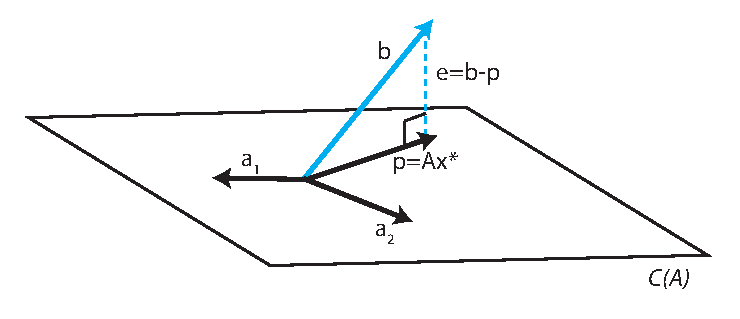
\includegraphics[width=12cm]{./least-squares.pdf}
 \caption{\label{fig:lsa}Least square approximation ($p$) for $b$ that minimizes error $e$. Plane is the column space of $A$ spanned by $a_1$ and $a_2$}
 \end{figure}
\begin{enumerate}
\setcounter{enumi}{113}
\item  LSA example for intersection of 3 non-intersecting lines: given $A, b$, want to find $\hat x$.

\begin{itemize}
\item Calculate $A ^{T} A, A ^{T} b$, and put these matrices' augmented matrix into rref to get values of $\hat x$
\end{itemize}

\item LSA example of fitting lines to data points (finding best fit for parameters $m,b$ in $y=mx+b$ notation)
\end{enumerate}
\subsection{Coordinates in different bases}
\label{sec-1_9}

\begin{enumerate}
\setcounter{enumi}{115}
\item  $V \subset \mathbb{R}^{n}, B=\{v_1,...,v_k\}$ is basis for $V$

\begin{itemize}
\item for all $a \in V, a= c_1 v_1 + ... + c_k v_k$
\item $c_1,c_2,\cdots,c_k$ known as `coordinates with respect to $B$'
\item $[a]_B= \begin{bmatrix}
                   c_1 & c_2 & \cdots & c_k \\
                   \end{bmatrix} ^{T} = c$, where scalar elements of $c$ are the weights of bases of $V$ that you need to get $a$ in terms of the basis vectors
\item Example: $[a]_B = \begin{bmatrix}
                           3 & 2 \\     
                         \end{bmatrix}  ^T \Rightarrow a=3 v_1 + 2 v_2$
\item Standard coordinates for $\mathbb{R}^{2}$  use ${\bf e}_1 = \begin{bmatrix}    
                                               1 & 0 \\         
                                             \end{bmatrix} ^{T}$, ${\bf e} _2 = \begin{bmatrix}    
                                                                                0 & 1 \\         
                                                                              \end{bmatrix} ^{T}$
\end{itemize}

\item $V \subset \mathbb{R}^{n}, B=\{v_1,...,v_k\}$ is basis for $V$:

\begin{itemize}
\item $C = \begin{bmatrix}              
              v_1 & v_2 & \cdots & v_k \\
            \end{bmatrix} ^{T} \in \mathbb{R}^{n \times k}$ is change of basis matrix for subspace $V$
\item \fbox{$a = C [a]_B$}: the basis vectors ($C$) multiplied by their weights ($[a]_B$) give the vector $a$ in standard coordinates
\end{itemize}

\item If $C$ (matrix with bases of $V$ in $B$ as column vectors) is invertible

\begin{itemize}
\item $C$ is square $\Rightarrow k \text{ (number of basis vectors) }=n \text{ (number of rows/dimension of basis vectors)} \Rightarrow \exists n$ basis vectors
\item $C$ has Linearly Independent columns
\item $B$ (set of basis vectors $\in \mathbb{R}^{n}$  for subspace $V$) is basis for $\mathbb{R}^{n}$
\item \fbox{$C$ invertible $\Leftrightarrow {\bf span} (B)= \mathbb{R}^{n}$}
\end{itemize}

\item Transformation matrix w.r.t. different basis; $T:\mathbb{R}^{n} \rightarrow \mathbb{R}^{n}$ ($T(x)= Ax$, $A$ transforms wrt standard basis). See Fig \ref{fig:transformation}

\begin{itemize}
\item \fbox{$D=C ^{-1} AC$}, where $D$ gets you from vector $a$ in terms of $B$ to transformation of $a$ in terms of $B$

\begin{itemize}
\item i.e., $D[ \vec{x} ]_B = [T( \vec{x})]_B$
\item \fbox{$A = CD C ^{-1}$}
\end{itemize}

\end{itemize}

\end{enumerate}
  \begin{figure}
  \begin{displaymath}
  \xymatrix{ \vec{x} \ar[r]^{A}_{CDC ^{-1} } \ar[d] _{C ^{-1} }
  & T(\vec{x}) \ar@<1ex>[d]_{C ^{-1} }  \\
  [\vec{x}]_B \ar@<-1ex>[u] _{C}  \ar[r]_{C ^{-1} AC}^{D}
  & *+[r]{[T( \vec{x} )]_B} \ar@<-2ex>[u]_{C}}
  \end{displaymath}
  \caption{Relationship of coordinate transformation matrices. $\vec{x}$ is a vector in standard coordinates, and $T( \vec{x} )=A \vec{x}$ is the transformation, in standard coordinates. These terms enclosed with brackets indicates the vector with respect to the basis $B$, whose elements form the columns of $C$. $C$ gets you from $B$ coordinates to standard coordinates, and the inverse reverses this.}
  \label{fig:transformation}
  \end{figure}
  % Sliding, here http://ftp.ktug.or.kr/tex-archive/macros/generic/diagrams/xypic/xy/doc/xyguide.pdf
\begin{enumerate}
\setcounter{enumi}{121}
\item  Example: Transformation that reflects across a line $L=\{c \hat u_1 : c \in \mathbb{R}\}$  (in $\mathbb{R}^{2}$)

\begin{itemize}
\item Use vector $\hat u_1= [1 \text{ }2] ^{T} = [[1 \text{ } 0] ^{T}]_B$ and $\hat u_2 = [2 \text{ } -1] ^{T} = [[0 \text{ } 1] ^{T}]_B$ (s.t. $\hat u_1 \perp \hat u_2$) as new basis vectors, which will be the columns of $C$
\item $A$ will have the transformations of the standard unit vectors ${\bf e} _{1}, {\bf e} _{2}$ as its columns (which are hard to find out)
\item $D$ will have the transformations of $\hat u _{1}, \hat u _{2}$ in modified coordinates as its columns

\begin{itemize}
\item this is easy: $\hat u _{1}$ will remain the same, $\hat u _{2}$ will be negated, i.e.,

\begin{itemize}
\item $[T(\hat u _{1} )]_B = [ \hat u _{1} ]_B = [ [1 \text{ } 0] ^{T} ]_B$
\item $[T(\hat u _{2} )]_B = [ -\hat u _{2} ]_B = [ [0 \text{ } -1] ^{T} ]_B$
\item These are column vectors of $D$
\end{itemize}

\end{itemize}

\item $A=CDC ^{-1}$
\end{itemize}

\end{enumerate}
\subsection{Orthonormal bases}
\label{sec-1_10}

\begin{enumerate}
\setcounter{enumi}{122}
\item  Orthonormal bases: basis vectors orthogonal and $\perp$ to each other
\item $B = \{v _{1} ,...,v_k\}$ is ON basis for $V, \vec{x} \in V \Rightarrow \vec{x} = c _{1} v _{1} + \cdots + c _{k} v _{k}$

\begin{itemize}
\item if $B$ is orthornormal basis, $v_i \cdot \vec{x} = c_i (v_k \cdot v_i) = c_i$, because of sifting property: $v_i \cdot v_j= \{i \ne j: 0, i=j: 1\}$
\item Remember weights for change of basis matrix
\end{itemize}

\end{enumerate}
\[
[ \vec{x} ]_B = \begin{bmatrix}
c_1 & c_2 & \cdots & c_k \\
\end{bmatrix} ^{T} =
\begin{bmatrix}                                             
v_1 \cdot x_1 & v_2 \cdot x_2 & \cdots & v_k \cdot x_k \\ 
\end{bmatrix}
\]
    \hspace{1.2cm} \textbullet{} so $[x]_b$ is easy to find
\begin{enumerate}
\setcounter{enumi}{124}
\item  $B=\{v _{1} ,v_2, ...,v_k\}$ is ON basis for subspace $V \subset \mathbb{R}^{n}$

\begin{itemize}
\item for $x \in \mathbb{R}^{n}, x = \vec{v} + \vec{w}$, where $\vec{v} = {\bf Proj} _{V} x \in V, \vec{w} = {\bf Proj} _{V ^{\perp} } x \in V ^{\perp}$
\item remember, \#109: \fbox{${\bf Proj} _V ( x) = Ay = A(A ^{T} A) ^{-1} A ^{T} x$}, where $A$ has basis vectors of subspace $V$ as its column vectors
\item if \fbox{$B$ is an ON basis}, $A ^{T} A=I_k$, because of ON sifting property (i.e., $A ^{T} = A ^{-1}$ )
\item \fbox{${\bf Proj} _V (x) = A A^{T} x$}
\end{itemize}

\setcounter{enumi}{127}
\item  Orthogonal matrices preserve angles and lengths (i.e., when ON matrix $C$ is used as a transformation matrix)

\begin{enumerate}
\item Length

\begin{itemize}
\item remember $y \cdot y= y ^{T} y$
\item with $\|x \| ^{2} = \| C x \| ^{2}$, the $C$ disappears because of above property
\end{itemize}

\item Angles

\begin{itemize}
\item look at $\cos \theta$ of 2 vectors from its relation to the dot product
\item compare this with $\theta$ between vectors $Cv, Cw$, keeping in mind preservation of length property above
\end{itemize}

\end{enumerate}

\item Gram-Schmidt process for basis $B= \{v_1, v_2, ..., v_k \}$ for subspace $V$

\begin{itemize}
\item basis not originally orthonormal, but first normalize $v_1$ (or any vector in the set): $u_1= v_1 / \| v_1\|$

\begin{itemize}
\item $\{u_1\}$ is now an ON basis for $V_1 = {\bf span } (v_1) \subset V$
\end{itemize}

\item $V_2 = {\bf span } (v_1,v_2)= {\bf span} (u_1,v_2) = {\bf span} (u_1, y_2)$, where $y_2 = v_2 - {\bf Proj} _{V_1} (v_2)$, i.e., $y_2$ is the element of $v_2$ that is orthogonal to $V_1$

\begin{itemize}
\item $y_2 = v_2 - (v_2 \cdot u_1) u_1$; $u_2$ is normalized version of $y_2$
\item $\{u_1, u_2\}$ is now ON basis for $V_2$
\end{itemize}

\item Repeat this for rest of vectors in $B$

\begin{itemize}
\item But, in general, $y_i = v_i - {\bf Proj} _{V_{1}} (v_i) - {\bf Proj} _{V_{2}} (v_i)- ... - {\bf Proj} _{V_{i-1}} (v_i) = v_i - (v_i \cdot u_1) u_1 - (v_i \cdot u_2) u_2 - ... - (v_i \cdot u_{i-1}) u_{i-1}$
\end{itemize}

\end{itemize}

\end{enumerate}
\subsection{Eigenvalues and vectors}
\label{sec-1_11}

\begin{enumerate}
\setcounter{enumi}{131}
\item  Eigenvalues; $T: \mathbb{R}^{n} \rightarrow \mathbb{R}^{n}$

\begin{itemize}
\item Remember, from \#122, a new basis was chosen for transformation $T$, s.t. $T$ did not scale basis vectors

\begin{itemize}
\item $T(v_1)= (1)v_1$
\item $T(v_2)= (-1)v_2$
\end{itemize}

\item For any transformation \fbox{$T: T(v)= Av= \lambda v$}

\begin{itemize}
\item $v$ is an eigenvector, and $\lambda \in \mathbb{R}$ is the eigenvalue associated with it
\end{itemize}

\end{itemize}

\item Finding $\lambda$, s.t. $Av=\lambda v$ :
\end{enumerate}
\begin{eqnarray}
    0 &=& \lambda v - Av \\
     &=& \lambda I_k v - Av  \\
     &=& (\lambda I_k - A)v  \\
     \Rightarrow v &\in& \mathcal{N}(\lambda I_k - A) = \{ x \in \mathbb{R}^{n} | B x = 0 \text{ where } (\lambda I_k - A)= B \} \\
    \text{Note: Columns of } D \text{ Linearly independent } &\Leftrightarrow& \mathcal{N}(D) = \{0\}
\end{eqnarray}
\hspace{1.2cm} \textbullet{} So, columns of $D$ must be Linearly Dependent for there to be a non-trivial eigenvector.

\hspace{1.2cm} \textbullet{} If columns LD, $D$ not invertible (since invertibility $\Leftrightarrow$ one-to-one/injective )

\hspace{1.2cm} \textbullet{} \fbox{$\Rightarrow {\bf Det} (\lambda I_k - A)= 0$ } should get you your eigenvalue
\begin{enumerate}
\setcounter{enumi}{133}
\item  Characteristic equation (in terms of $\lambda$) is found by evaluating the determinant: \textbf{Det} $(\lambda I_k - A)= 0$
\item Find eigenvector: Solve for $v$ in $(\lambda I_n - A) v = 0$

\begin{itemize}
\item Won't need to do rref on augmented matrix, since the RHS is the zero vector
\item rref $(\lambda I_n - A)$ will give elements of $v$
\item \textbf{Eigenspace} will be the span of the eigenvectors
\end{itemize}

\setcounter{enumi}{137}
\item  Eigenbasis (basis composed of eigenvectors) make good coordinate system

\begin{itemize}
\item $A \in \mathbb{R}^{n \times n}$ has $n$ LI eigenvectors, $B=\{v_1, v_2, ..., v_n\}$

\begin{itemize}
\item $n$ vectors that are LI $\Rightarrow B$ is basis for $\mathbb{R}^{n}$
\item $Av_1 = \lambda_1 v_1 + 0 v_2 + ... + 0 v_n; Av_2 = 0 v _{1} + \lambda_2 v_2 + ... + 0 v_n$ (and you get the idea)
\item Remember chart from \#122: vectors in $B$ will form columns of $C$
\item Find column $j$ of $D$ by doing $[T(v_j)]_B = [0 \text{ } 0 \cdots \lambda_j \cdots 0 ]^T = [d_1 \text{ } d_2 \cdots d_n] [0 \text{ } 0 \cdots 1 \cdots 0] ^{T}$
\end{itemize}

\end{itemize}

\end{enumerate}
\[
\text{Thus, }D=
\begin{bmatrix}
  \lambda_1 &         0 & \cdots &         0 \\
          0 & \lambda_2 & \cdots &         0 \\
     \vdots &    \vdots & \ddots &    \vdots \\
          0 &         0 & 0      & \lambda_n \\
\end{bmatrix}
\]
Easy to apply transformation on a whole range of input vectors, and can be worth the overhead of getting the basis and $D$, if you want to scale up.
\section{Appendix}
\label{sec-2}
\subsection{Why reduced row echelon works}
\label{sec-2_1}

We can use reduced row echelon form to solve a system of equations $Ax=b$. We want to know any of the polynomials of degree $n \le 2$ that go through the points $\{ (1,-1), (2,3), (3,3)\}$. We will look for coefficients $a_i$ associated with terms $x^i$. Matching the $x^i$ values with their respective coefficients and $y$ values gives us the system
 \begin{eqnarray}
 \label{eqn:linsys1}
   a_0 + a_1 + a_2 &=& -1 \\
   a_0 + 2a_1 + 4a_2 &=& 3 \\
   a_0 + 3a_3 + 9a_2 &=& 3
 \label{eqn:linsys3}
 \end{eqnarray}
which can be represented in $Ax=b$ form by
$$
\begin{bmatrix}
  1 & 1 & 1 \\
  1 & 2 & 4 \\
  1 & 3 & 9 \\
\end{bmatrix}
\begin{bmatrix}
  a_0 \\
  a_1 \\
  a_2 \\
\end{bmatrix}
=
\begin{bmatrix}
  -1 \\
   3 \\
   3 \\
\end{bmatrix}.
$$ 
We can see from Eqns. \eqref{eqn:linsys1}-\eqref{eqn:linsys3} that our method should be to perform elementary row operations on the different equations, in order to ultimately have only a single unique $a_i$ term on the LHS of each equation. We want the $a_i$ terms to remain in the same columns, but the coefficients to mostly cancel each other. Thus we will augment matrices $A$ and $b$, and get them in reduced row echelon form:
$$
{\bf rref} \left(
\begin{bmatrix}
  1 & 1 & 1 & -1 \\
  1 & 2 & 4 &  3 \\
  1 & 3 & 9 &  3 \\
\end{bmatrix}
\right) =
\begin{bmatrix}
  1 & 0 & 0 & -9 \\
  0 & 1 & 0 & 10 \\
  0 & 0 & 1 & -2 
\label{solved}
\end{bmatrix}
$$
Un-augmenting this matrix, we see that it corresponds to the equations
\begin{eqnarray}
  a_0 &=& -9 \\
  a_1 &=& 10 \\
  a_2 &=& -2
\end{eqnarray}
so that the polynomial can be given as $y(x) = -9 + 10x -2 x ^{2}$.

Note, if the last row of the matrix \ref{solved} had been $[ 0 \text{ } 0 \text{ } 0 \text{ } 1]$, meaning that $0 a_0 + 0 a_1 + 0 a_2 = 1$, (an obvious contradiction), it would indicate that there is no possible polynomial of this degree that passes through all the points.
\subsection{Solving an example nullspace using reduced row echelon form (\#35)}
\label{sec-2_2}

Let's find the nullspace for a matrix
\[
A=
\begin{bmatrix}
  1 & 1 & 1 & 1 \\
  1 & 2 & 3 & 4 \\
  4 & 3 & 2 & 1 \\
\end{bmatrix}
\]
Remember, $\mathcal{N}(A) = \{x \in \mathbb{R}^{n}: Ax = 0\}$. So we will look for the vector $x \in \mathbb{R}^{4}$ below:
\[
\begin{bmatrix}
  1 & 1 & 1 & 1 \\
  1 & 2 & 3 & 4 \\
  4 & 3 & 2 & 1 \\
\end{bmatrix}
\begin{bmatrix}
  x_1 \\
  x_2 \\
  x_3 \\
  x_4 \\
\end{bmatrix}
=
\begin{bmatrix}
  0 \\
  0 \\
  0 \\
\end{bmatrix}
\]
We will solve this linear system of equations by putting the following matrix into reduced row echelon form:
\[
\begin{bmatrix}
  1 & 1 & 1 & 1 & 0\\
  1 & 2 & 3 & 4 & 0\\
  4 & 3 & 2 & 1 & 0\\
\end{bmatrix}
\]
This is essentially the same as putting the unaugmented matrix $A$ into RREF, since there is no elementary row operation that will change the elements in the last column, but either way it gives us
\[
\begin{bmatrix}
  1 & 0 & -1 & -2 & 0 \\
  0 & 1 &  2 &  3 & 0 \\
  0 & 0 &  0 &  0 & 0 \\
\end{bmatrix}
\]
The first two rows/columns have pivot elements, whose columns are the pivot columns (since they have leading 1's). The rest are free columns. The matrices can be read to be saying
\begin{eqnarray}
x_1 &=& x_3 + 2 x_4 \\
x_2 &=& -2 x_3 - 3 x_4
\end{eqnarray}
Or,
\[
\begin{bmatrix}
  x_1 \\
  x_2 \\
  x_3 \\
  x_4 \\
\end{bmatrix}
= x_3
\begin{bmatrix}
  1  \\
  -2 \\
  1  \\
  0  \\
\end{bmatrix}
+ x_4
\begin{bmatrix}
   2 \\
  -3 \\
   0 \\
  1  \\
\end{bmatrix}
\]
And since, in general, $\mathcal{N}(A)= \mathcal{N}( {\bf rref} (A))$, we get
\[
\mathcal{N}(A) = {\bf span} \left(
\begin{bmatrix}
  1  \\
  -2 \\
  1  \\
  0  \\
\end{bmatrix}
,
\begin{bmatrix}
   2 \\
  -3 \\
   0 \\
  1  \\
\end{bmatrix}
\right).
\]
\subsection{Invertibility implications}
\label{sec-2_3}

For an $n$-by-$n$ matrix $A$ 

\begin{center}
\begin{tabular}{ll}
 Invertible                                &  mnemonic                                                                                 \\
\hline
 $\vert A\vert \ne 0$                      &  $\vert A\vert = 0$ $\Rightarrow$ you can't compute the inverse                           \\
 non-singular                              &  - (remember base case 2 \texttimes{} 2 matrix inverse involves $1/\vert A\vert$ term)    \\
 $A$ is full rank                          &  linearly independent columns (invertibility $\Rightarrow$ 1-to-1/injective)              \\
 $\mathcal{N}(A)=\{0\}$                    &  linearly independent columns                                                             \\
 $\mathcal R (A)= \mathbb{R}^{n}$          &  linearly independent columns                                                             \\
 $Ax=b$ has unique solution for every $b$  &  - no more than one solution (can't add members of $\mathcal N (A)$ for multiple $b$)     \\
                                           &  - one solution, since $\mathcal R (A)= \mathbb{R}^{n}$; everything reachable/surjective  \\
                                           &  - one solution found using the unique inverse of \emph{A}                                \\
 rref($A)=I_n$                             &                                                                                           \\
 $A$ is a product of elementary matrices   &                                                                                           \\
\end{tabular}
\end{center}

\end{document}